\subsection{Описание предложенного подхода}
Для решения задачи, поставленной в пункте~\ref{formulation} в данной работе предлагается подход, основанный на введении в облачную систему дополнительного сервиса как показано на рис.~\ref{suggested-approach}.
Такой сервис будет называться далее сервисом управления виртуализированной инфраструктурой.

\begin{figure}[hbtp]
    \centering
    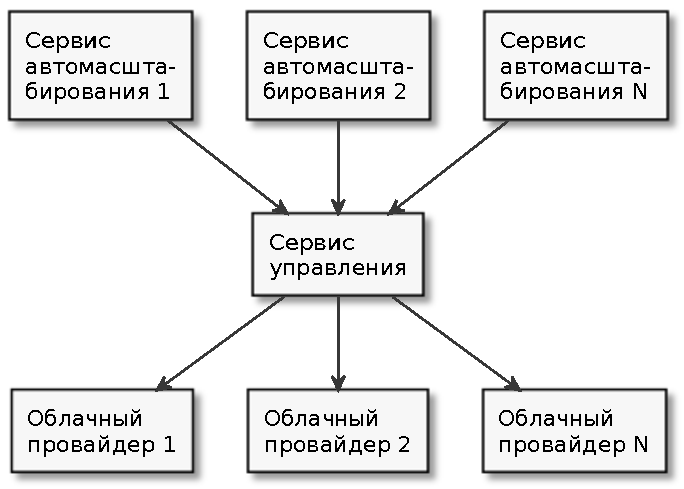
\includegraphics[width=10cm]{img/suggested-approach.pdf}
    \caption{Облачная система с дополнительным сервисом управления}
    \label{suggested-approach}
\end{figure}

При помощи введения в систему дополнительного промежуточного компонента решается задача абстрагирования компонентов управления ресурсами от конкретных объектов управления - платформ виртуализации инфраструктуры. 
Таким образом, при разработке компонента управления ресурсами (например, сервиса автомасштабирования), нужно будет учитывать только программный интерфейс (API) сервиса управления, даже если в целевой системе будет несколько различных платформ облачных вычислений.

Тем не менее, при необходимости введения в систему новой платформы виртуализации, возникнет необходимость доработки сервиса управления с учётом программного интерфейса добавляемой платформы.
Однако это потребуется сделать лишь один раз и далее можно будет использовать неограниченное количество облачных платформ, предоставляющих такой же программный интерфейс.

\FloatBarrier 

\subsection{Аутентификация в управляемых платформах}
В целях уменьшения затрат на реализацию компонентов управления ресурсами, аутентификацию в управляемой системе должен выполнять тоже сервис управления.
Для этого у администратора системы должна быть возможность сохранить параметры подключения, такие как логин, пароль, токен и так далее. 
После сохранения параметров, администратору системы должен быть предоставлен идентификатор сохранённого набора параметров.
После этого администратор должен будет передать этот идентификатор компоненту управления ресурсами.
Дальнейшее взаимодействие с сервисом управления потребует от клиентов только идентификатора.
Таким образом, реализация компонента управления ресурсами не будет требовать реализации процесса аутентификации ни в одной из целевых платформ виртуализации.

Как проиллюстрировано на рис.~\ref{saving}, после начальной конфигурации компонентов системы, участие администратора в работе системы не требуется.
Для взаимодействия с сервисом управления, компоненту управления требуется знать лишь идентификатор, имея который есть возможность осуществлять, например, горизонтальное масштабирование.

\begin{figure}[hbtp]
    \centering
    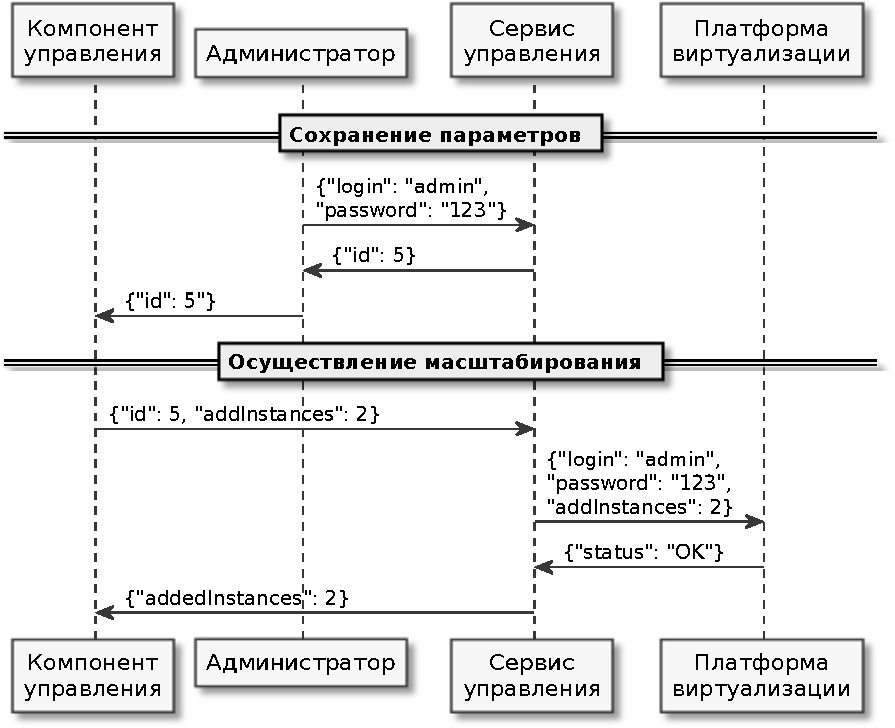
\includegraphics[width=\textwidth]{img/saving.pdf}
    \caption{Пример конфигурации компонента управления и дальнейшего взаимодействия}
    \label{saving}
\end{figure}
